\section{Connected components \& the fundamental groupoid I}

Lecture 12.11

For references for this section see \cite[Sections 1.2.1, 1.1.4 \& 1.2.4]{kerodon}.

Consider the following functors
\[
\begin{tikzcd}
    \Set 
    \arrow[r, hook, bend left, "\iota" pos= 0.55,""{name=A, above}]
    &
    \Gpd
    \arrow[l, bend left ,"\pi_0" pos=0.4,""{name=B, above}]
    \ar[from=A, to=B, symbol=\dashv]
    \ar[r, bend left, "j",""{name=E, above}]
    &
    \Cat
    \ar[l, bend left, "L" pos=0.6,""{name=F, below}]
    \ar[from=E, to=F , symbol=\dashv]
    \ar[r, hook, bend left, "N",""{name=C, above}]   
    &
    \Set_{\Delta}
    \ar[l, bend left, "\tau" pos= 0.45,""{name=D, below}]
    \ar[from=C, to=D , symbol=\dashv] 
\end{tikzcd}
\]

These functors admit left adjoints:
Given $G \in \Gpd$ we let $\pi_0(G) \in \Set$ be its set of isoclasses.

\begin{prop}
    The canonical functor  $G \to \iota(\pi_0(G))$, $G \in \Gpd$ are the components of the unit of an adjunction 
    \[
    \begin{tikzcd}
        \pi_0\colon \Gpd 
        \ar[r,shift left]
        &
        \Set : \iota
        \ar[l,shift left, "\adj" ]
    \end{tikzcd}
    \]
\end{prop}

\begin{proof}
    Let $J \in \Set$ and let $F$ be a functor $F \colon G \to \iota(J)$. We observe that $\forall f \colon X \to Y$ in $G$ we have $F(f) = \id_{F(x)}=\id_{F(y)}$
    in other words, $F$ is a constant on isomorphism-classes in $G$, hence $F$ factors uniquely through $G \xrightarrow{\eta_g} \iota(\pi_0(G))$.
    \[
    \begin{tikzcd}
        G 
        \ar[r,"\eta_g"]
        \ar[rd, "\forall F"']
        &
        \iota(\pi_0(G))
        \ar[d,"\iota(\Bar{F})"]
        \\
        &
        \iota(J)
    \end{tikzcd}
    \]
    This gives an isomorphism $\Hom_{\Set}(\pi_0(G),-) \cong \Hom_{\Gpd}(G,\iota(-))$, which means we have an adjunction $\pi_0 \dashv \iota$ with unit $\eta$.
\end{proof}

For $\mathcal{C} \in \Cat$ we define $L\mathcal{C} \in \Gpd$ as follows:
Consider the quiver with vertices $\Ob(\mathcal{C})$ and arrows $\Mor(\mathcal{C}) \amalg \{ f^{-} \mid f \in \Mor(\mathcal{C}) \}$.
For $f \in \Mor(\mathcal{C})$
\begin{center}
\begin{tabular}{cc}
    $s(f)=$ domain $f$ & $X \xrightarrow{f} Y$  
    \\
    $t(f)=$ codomain of $f$ &
    \\
    $s(f^{-})=$ codomain of $f$ & $X \xleftarrow{f^{-}}Y$
    \\
    $t(f^{-})=$ domain of $f$
\end{tabular}
\end{center}

Consider the quotient of the path category of the above quiver by the relation generated by 
\begin{itemize}
    \item 
    $\forall X \in \Mor(\mathcal{C}), \id_X \sim e_X\colon $ lazy path at $X$
    \item 
    $\forall f,g \in \Mor(\mathcal{C})$ composable $\cdot \xrightarrow{f} \cdot \xrightarrow{g} \cdot \sim \cdot \xrightarrow{g \circ f} \cdot$
    \item 
    $\forall f \in \Mor(\mathcal{C})$
    \begin{align*}
        \cdot \xrightarrow{f} \cdot \xrightarrow{f^-} \cdot \sim \id
        \\
        \cdot \xrightarrow{f^-} \cdot \xrightarrow{f} \cdot \sim \id
    \end{align*}
    that is $[f^-]=[f]^{-1}$
\end{itemize}

\begin{thm}
    The canonical functors $\gamma = \gamma_{\mathcal{C}}\colon \mathcal{C} \to L \mathcal{C}$, $\mathcal{C} \in \Cat$, form the components of the unit of an adjunction
    \[
    \begin{tikzcd}
        L\colon \Cat
        \ar[r]
        &
        \Gpd:j
    \end{tikzcd}
    \]
\end{thm}

\begin{proof}
    A functor $F \colon \mathcal{C} \to j(G)$, $G \in \Gpd$ nessecarily inverts all maps in $\mathcal{C}$ hence the functor $\Bar{F}(x) \coloneqq F(x)\colon L\mathcal{C} \to j(G)$ $F(f) \coloneqq F([f])$ $\Bar{([f^-])\coloneqq F(f)^{-1}}$ is well defined and is the unique functor such that 
    \[
    \begin{tikzcd}
        \mathcal{C} 
        \ar[r, "\gamma_{\mathcal{C}}"]
        \ar[dr, "F"']
        &
        j(L\mathcal{C})
        \ar[d, "j(\Bar{F})"]
        \\
        &
        j(G)
    \end{tikzcd}
    \]
    commutes, giving $L \dashv j$ with unit $\eta$.
\end{proof}

    Consider now for $X \in \Set_{\Delta}$, the quiver with vertices $X_0$ and arrows $X_1$ with $d_1=s\colon, X_1 \to X_0$ and $d_0= t\colon X_1 \to X_0 $. We have that $\tau(X)$ is the quotient of the path category of this quiver modulo the relation 
    \[
    \begin{tikzcd}
        &
        {}
        \ar[rd, "f_{21}"]
        &
        \\
        {}
        \ar[ru, "f_{10}"]
        \ar[rr, "f_{20}"']
        &
        &
        {}
    \end{tikzcd}
    \in X_2
    \implies 
    [f_{20}]=[f_{21}] \circ [f_{10}].
    \]   
    

\begin{prop}
    The canonical maps $\eta_X\colon X \to N(\tau X)$ ,  $X \in \Set_{\Delta}$ form the components of the unit of an adjunction 
    \[
    \begin{tikzcd}
        \tau\colon \Set_{\Delta}
        \arrow[r, shift left]
        &
        \Cat\colon N
        \arrow[l, shift left, "\adj"]
    \end{tikzcd}
    \]
\end{prop}

\begin{defi}
    We also have the composite adjunction
    \[
    \begin{tikzcd}
        \Set 
        \arrow[r, hook, bend left, "\iota" pos= 0.55,""{name=A, above}]
        \ar[rrr, bend right=50, ""]
        &
        \Gpd
        \arrow[l, bend left ,"\pi_0" pos=0.4,""{name=B, above}]
        \arrow[from=A, to=B, symbol=\dashv]
        \arrow[r, bend left, "j",""{name=E, above}]
        &
        \Cat
        \arrow[l, bend left, "L" pos=0.6,""{name=F, below}]
        \arrow[from=E, to=F , symbol=\dashv]
        \arrow[r, hook, bend left, "N",""{name=C, above}]   
        &
        \Set_{\Delta}
        \arrow[l, bend left, "\tau" pos= 0.45,""{name=D, below}]
        \ar[lll, bend right=50, "\mathbb{\pi}_0"']
        \arrow[from=C, to=D , symbol=\dashv] 
    \end{tikzcd}    
    \]
    \begin{tikzcd}
        \pi_0\coloneqq \pi_0 \circ L \circ \tau \colon \Set_{\Delta}
        \arrow[r, shift left]
        &
        \Cat\colon N \circ j \circ \iota
        \arrow[l, shift left, "\adj"]
    \end{tikzcd}
\end{defi}

\begin{defi}
    For $ X \in \Set_{\Delta}$ we call $\pi_0(X)\in \Set$ is a \underline{connected component}.
    For $ I \in \Set$ we have that
    \[
    N(j(\iota(I)))_n=N(\iota(I))_n=\Hom_{\Cat}([n], \iota(I)) \cong I
    \]
    which means that 
    \[
    N \circ j \circ \iota = \const_{\Delta}
    \]
    By uniqueness of adjoints we obtain that $\pi_0 \cong \colim_{\Delta}$ is adjoint to $\const_{\Delta} \cong N \circ j \circ \iota$ where $\pi_0(X)\cong X_0 / \sim$ and $X \sim Y$ if and only if there exists a zigzag of edges in $X$.
    Consider now the composite adjunction
\end{defi}
    \[
    \begin{tikzcd}
        \Gpd
        \arrow[r, bend left, "j",""{name=A, above}]
        \arrow[rr, bend left=50, "\pi_1"]
        &
        \Cat
        \arrow[l, bend left ,"L" pos=0.45,""{name=B, above}]
        \arrow[from=A, to=B, symbol=\dashv]
        \arrow[r, bend left, "N",""{name=C, above}]
        &
        \Set_{\Delta}       
        \arrow[l, bend left ,"\tau" pos=0.45,""{name=D, above}]
        \arrow[from=C, to=D, symbol=\dashv]
        \arrow[ll, bend left=55, "N"]
    \end{tikzcd}
    \]
    Where 
    \begin{tikzcd}
        \pi_1\coloneqq L \circ \tau \colon \Set_{\Delta}
        \arrow[r, shift left, "\Gpd"]
        &
        \Gpd \colon N \circ j = N_{\mid \Gpd}=N
        \arrow[l, shift left, "\adj"]
    \end{tikzcd}

\begin{defi}
    For $X \in \Set_{\Delta}$ we call $\pi_1(X)\in \Gpd$ its \underline{fundamental groupoid}.
    For $x \in X_0$ we define $\pi_1(X,x) \in \Grp$ as 
    \[
    s_0(x)=[1_x] \in \Hom_{\pi_1(X)}(x,x)
    \]
    Let $f \colon X \to Y$ in $\Set_{\Delta}$ be a morphism then we get a functor $\pi_1(X) \to \pi_1(Y)$ given as 
    \[
    \begin{tikzcd}
        \pi_1(f)\colon \pi_1(X,x)=\Hom_{\pi_1(X)}(x,x)
        \arrow[r]
        &
        \Hom_{\pi_1(Y)}(f_0(x),f_0(x))=\pi_1(Y,f_0(x))
    \end{tikzcd}
    \]
\end{defi}

Lecture:14.11 

\subsection{connected component}

We have the adjunction $\pi_0 \colon \SetD$
\[
\begin{tikzcd}
    \pi_0(X)\cong \coeq(X_1
    \arrow[r, shift left, "d_1"]
    \arrow[r, shift right, "d_0"']
    &
    X_0)
\end{tikzcd}
\]
For $X \in \Set_{\Delta}$ we have the unit morphism $\eta_X \colon X \to \pi_0(X)$.
When $\eta_X$ is an isomorphism we say that $X$ is \underline{discrete}.



We want to show that $X \in  \Set_{\Delta}$ decomposes as the disjoint union of the connected simplicial subsets, called its \underline{connected components}.

\begin{construction}
    For $C \in  \pi_0(X)=X_0/\sim$ ( in particular $C \subseteq X_0$) let $X(C)_n \coloneqq \{ \sigma  \in X_n \mid \forall \Delta \xrightarrow{f}\Delta^n \xrightarrow{\sigma}X , \sigma \circ f\in C\}$.
    Notice that $X(C) \subseteq X$ is a simplicial subset since for $\sigma  \in X(C)_n$ and $\tau \colon \Delta^m \to \Delta^n$ we have that 
    \[
    \begin{tikzcd}
        \Delta^m
        \arrow[r,"\tau"]
        &
        \Delta^n
        \arrow[r,"\sigma"]
        &
        X
        \\
        \Delta^0
        \arrow[u,"v"]
        \arrow[ru]
    \end{tikzcd}    
    \]
\end{construction}

Moreover, $X(C) \subseteq X$ is a summand in the sense that $X \cong X(C) \amalg (X \setminus X(C))$ for $X_n \setminus X(C)_n$ also defines a simplicial subset.
\[
X_n\setminus X(C)_n =\{ \sigma  \in X_n \mid \forall \Delta \xrightarrow{f}\Delta^n \xrightarrow{\sigma}X,\sigma\circ f \notin C\}
\]

\begin{prop}
    The canonical map 
    \[
    \begin{tikzcd}
        \amalg_{C \in \pi_0(X)}X(C)
        \arrow[r, hook]
        &
        X
        \\
        X(C)
        \arrow[u, hook]
        \arrow[ru, "\iota_C"]
    \end{tikzcd}
    \]
    is an isomorphism of simplicial sets.
\end{prop}

\begin{rmk}
    Notice that
    $\pi_0(X(C))=\{C\}$ as well as 
    $\amalg_{C \in \pi_0(X)}\pi_0(X(C))
    =\pi_0(\amalg_{C \in \pi_0(X)}X(C)) 
    \isomorphism 
    \pi_0(X)$
\end{rmk}

\begin{prop}
    For any simplicial set $X \in \Set_{\Delta}$, that is not equal to the empty set, the following are equivalent 
    \begin{enumerate}
        \item 
        $\pi_0(X)=\{*\}$
        \item 
        if $X \cong Y \amalg Z$ then $Y = \emptyset$ or $Z = \emptyset$
    \end{enumerate}
    When this is the case we call $X$ \underline{connected}.
\end{prop}

\begin{proof}
    \begin{enumerate}
        \item 
        $''1)\implies2)''$
        We argue by contrapositive. 
        Let
        \[
        X \cong Y \amalg Z
        \] 
        such that neither $Y$ nor $Z$ are the empty simplicial set.
        Then we have that 
        \[
        \pi_0(X) \cong \pi_0(Y) \amalg \pi_0(Z) \neq \{ *\}
        \]
        \item 
        $''1)\implies2)''$
        We argue again by contrapositive. 
        \[
        \amalg_{C \in \pi_0(X)} X(C) \isomorphism X
        \]
        where at least two of the summands on the left are nonempty.
    \end{enumerate}
\end{proof}

\begin{prop}
    Let $\emptyset \neq X \in \Set_{\Delta}$ and $S\subseteq X$ a connected component, that is $\pi_0(S)=\{*\}$ and $X=S \amalg (X \setminus S)$.
    Then $\exists!C \in \pi_0(X)$ such that $S=X(C)$.
\end{prop}

\begin{prop}
    Let $X,Y$ be connected simplicial sets then $X  \times Y$ is connected. 
\end{prop}

\begin{proof}
    Let $(x,y),(x',y') \in (X\times Y)_0=X_0 \times Y_0$ and $X \xleftarrow{f}X''\xrightarrow{g}X'$ with $f,g \in X_1$ as well as $y \xrightarrow{h} y'$ with $h \in Y_1$.
    \[
    \begin{tikzcd}
        (x,y)
        \arrow[d,"{( 1_x , h )}"']
        &
        (x',y')
        \\
        (x,y')
        &
        (x'',y)
        \arrow[l, "{(f,1_{y'})}"]
        \arrow[u, "{(g,1_{y'})}"']
    \end{tikzcd}
    \]
    \begin{Warning}
        The collection of simplicial sets is not closed under infinite products.
        Take the nerve of the natural numbers $ N ( \mathbb{ N } ) $ as well ordered set and let $ X $ be the associated simplicial set, then $ S = \prod_{ n \in \mathbb{ Z }_{ \geq 0 } } X $ is not connected, since the element $ i = ( 0 , 0 , 0 ,\dotsc ) $ and $ j = ( 0 , 1 , 2 , 3 , \dotsc ) $ have no edge between one another, since edges in the product are finite compositions of tuples of edges in the components.
    \end{Warning}
\end{proof}

\begin{comment}
    
\section{boundaries and horns}

Let $X \in \Set_{\Delta}$ and $f,g \in X_1$ such that $d_0f=d_1g$, that is we have the following 
\[
d_1f\xrightarrow{f}d_0f=d_1g\xrightarrow{g}d_0g
\]
We would like to have a composite of $f$ and $g$, that is a commutative diagramm
\[
\begin{tikzcd}
    &
    a
    \arrow[rd, "g"]
    &
    \\
    b
    \arrow[ru, "f"]
    \arrow[rr, "n"']
    &
    &
    c
\end{tikzcd}
\in X_2
\]
We introduce the 2-horn at position 1 $\Lambda_1^2 \subseteq \Delta^2$ as the simplicial subset generated by $0 \xrightarrow{01}1$ and $1 \xrightarrow{12}2$, that is 
\[
\begin{tikzcd}
    &
    1
    \arrow[dr]
    &
    \\
    0
    \arrow[ur]
    &&
    2
\end{tikzcd}
=
\Lambda_1^2 
\xrightarrow{(f,g)}
X
\]
with $f,g \in X_1$ and $d_0f=d_1g$

\[
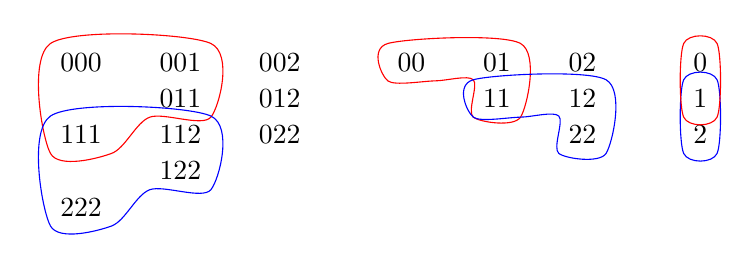
\begin{tikzpicture}
    \matrix[column sep = 0.5cm]
    {
    \node(000) {000};& \node(001) {001};& \node{002};&;& \node(00){00};& \node(01){01};& \node{02};&;& \node(0){0};\\
    &\node(011){011};& \node{012};&;&;& \node(11){11};& \node(12){12};&;& \node(1){1};\\
    \node(111){111};& \node(112){112};& \node{022};&;&;&;& \node(22){22};&;&\node(2){2};\\
    &\node(122){122};\\
    \node(222){222};\\
    };
    \draw [blue] plot [smooth cycle] coordinates { (1.north west) (1.north east) (2.south east) (2.south west)};
    \draw [red] plot [smooth cycle] coordinates { (0.north west) (0.north east) (1.south east) (1.south west)};
    \draw [red] plot [smooth cycle] coordinates { (00.north west) (01.north east) (11.south east) (11.south west) (11.north west) (00.south east) (00.south west)};
    \draw [blue] plot [smooth cycle] coordinates { (11.north west) (12.north east) (22.south east) (22.south west) (22.north west) (11.south east) (11.south west)};
    \draw [red] plot [smooth cycle] coordinates { (000.north west) (001.north east) (011.south east) (011.south west) (111.south east) (111.south west) };
    \draw [blue] plot [smooth cycle] coordinates { (111.north west) (112.north east) (122.south east) (122.south west) (222.south east) (222.south west) };
\end{tikzpicture}
\]

\[
\text{pushout:}
\begin{tikzcd}
    \Delta^0=\Delta^{\{1\}}
    \arrow[r,hook]
    \arrow[d,hook]
    &
    \Delta^{\{0,1\}}
    \arrow[d,"01"]
    \arrow[rdd,bend left]
    &
    &
    \\
    \Delta^{\{1,2\}}
    \arrow[rrd, bend right]
    \arrow[r, "12"]
    &
    \Lambda^2_1
    \arrow[rd,dashed,"\exists!"]
    &
    &
    \\
    &
    &
    X
\end{tikzcd}
\]

\todo{fill in the missing}
\end{comment}

\subsection{Exercises}

\begin{Exercise}
    Recall that we defined the connected component functor $ \pi_0 : \SetD \to \Set $ as 
    \[
        \pi_0 ( X ) \coloneqq \colim_{ \Delta } X 
    \]
    which yields a left adjoint to the constant diagram functor $ \const : \Set \to \SetD $.
    
    \begin{enumerate}[label=(\alph*)]
        
        \item 
        Show that $ \pi_0 ( \Delta^n ) $ is a one point set for any $ n \in \mathbb{ N } $.
    
        \item 
        Recall from Exercise 6.2 the boundaries $ \partial \Delta^n $ and horns $ \Lambda_k^n $ of $ \Delta^n $.
        Compute $ \pi_0 ( \partial \Delta^n ) $ and $ \pi_0 ( \Lambda_k^n ) $. 
    \end{enumerate}
    
    By definition the connected components of a small category $ \mathcal{ C }$ are defined as the coequalizer 
    \[
        \begin{tikzcd}
        \Mor ( \mathcal{ C } ) 
        \ar[r, shift left, "\text{target}"]
        \ar[r, shift right, "\text{source}"']
        &
        \Ob( \mathcal{ C } )
        \end{tikzcd}
    \]
    
    \begin{enumerate}[label=(\alph*), resume]
       
        \item 
        Show that for any simplicial set $ X $, the connected components $ \pi_0 ( X ) $ of $ X $ agree with the connected components of the category of elements $ \int^{ \Delta } X $.
    
        \item 
        Show that the connected components of a category $ \mathcal{ C } $ agree with the connected components of its nerve $ \pi_0 ( N ( \mathcal{ C } ) )$.
        
    \end{enumerate}
\end{Exercise}

\begin{Exercise}
    For a simplicial set $ X $, let $\bold{ Sk_n } ( X ) $ be the smallest simplicial subset of $ X $ such that $ ( \bold{ Sk_n } ( X ) )_m = X_m $ for $ m \leq n $.
    
    \begin{enumerate}
        \item 
        Show that there is a natural isomorphism $ \bold { Sk_n } ( X ) \cong \bold { sk_n } ( X ) $, i.e. $ \bold{ Sk_n } $ describes the $n$-skeleton functor from Exercise 6.2.
    \end{enumerate}
    
    Consider for any simplicial set $ X $ the canonical functor $ \bold{ sk }_X \colon \mathbb{ N }_0 \to \SetD $ with $ \bold{ sk }_X ( n ) \coloneqq \bold{ sk }_n ( X ) $ and morphisms induced by the inclusion $ \bold{ sk }_n ( X ) \subseteq X $.
    We call the image of $ \bold{ sk }_X $ the skeletal filtration of $ X $. 
    For convenience, we set $ \bold{ sk }_{-1} ( X ) $ to the empty presheaf.
    
    \begin{enumerate}[label=(\alph*), resume]
        \item 
        Argue that the morphisms in the skeletal filtration of $ X $ are monomorphisms and show that $ X \cong \colim_{ \mathbb{ N } } \bold{ sk }_X$.
    
        \item 
        Recall that $ \sigma \in X_n $ can be viewed as a morphism $ \sigma : \Delta^n \to X $.
        Observe that $ \sigma $ factors through $ \bold{ sk }_n ( X ) $ and that the precomposition of $ \sigma $ with the inclusion $ \partial \Delta^n \subseteq \Delta $ factors through $ \bold{ sk }_{n-1} ( X ) $.
        Show that these maps assemble into a pushout diagram.
        \[
        \begin{tikzcd}
            \coprod_{ \sigma \in X_n^{nd}} \partial \Delta^n
            \rar
            \dar
            &
            \coprod_{ \sigma \in X_n^{nd}} \Delta^n
            \dar
            \\
            \bold{sk_{n-1}}(X)
            \rar
            &
            \bold{sk_n}(X)
        \end{tikzcd}
    	\]
        Here $X_n^{nd} \coloneqq X_n \setminus ( \bold{ sk_{n-1} ( X ) })_n$ 
        denotes the set of non-degenerate $n$-simplicies in $ X$
    
        \item   
        Show that the geometric realisation of a simplicial set is a CW complex.
    \end{enumerate}
\end{Exercise}


